%%%%%%%%%%%%%%%%%%%%%%% file moduleX_template.tex %%%%%%%%%%%%%%%%%
%
%
% This is a template for creating your papers for the course KRW
% It is based on the standard Latex template for Springer publications
% but contains a suggestion for the structure and some content of the 
% paper. 
%
% Please adapt this document wherever needed.
%
% For more information about the required Latex Style check the document
% typeinst.pdf in the StyleFiles directory. 
%
%%%%%%%%%%%%%%%%%%%%%%%%%%%%%%%%%%%%%%%%%%%%%%%%%%%%%%%%%%%%%%%%%%%%%%%%%


\documentclass[runningheads,a4paper]{../../StyleFiles/llncs}

\usepackage{url}
\usepackage{graphicx}
\usepackage{amssymb}
\usepackage{listings}
\lstset{language=SQL,morekeywords={PREFIX,java,rdf,rdfs,url}}
 

\newcommand{\keywords}[1]{\par\addvspace\baselineskip
\noindent\keywordname\enspace\ignorespaces#1}

\begin{document}

\mainmatter  % start of an individual contribution

% first the title is needed
\title{Data- and Systems Paper : Finding events}

% a short form should be given in case it is too long for the running head
\titlerunning{Data- and Systems Paper}

% the name(s) of the author(s) follow(s) next
%
% NB: Chinese authors should write their first names(s) in front of
% their surnames. This ensures that the names appear correctly in
% the running heads and the author index.
%
\author{Alivanistos, Dimitris. \\ Baez, Selene. \\ Jemmett, Andrea. }
%
\authorrunning{Alivanistos, Dimitris. \\ Baez, Selene. \\ Jemmett, Andrea.}
% (feature abused for this document to repeat the title also on left hand pages)

% the affiliations are given next; don't give your e-mail address
% unless you accept that it will be published
\institute{\url{d.alivanistos@student.vu.nl} \and \url{s.baezsantamaria@student.vu.nl} \and \url{a.jemmett@student.vu.nl}}

\maketitle


\begin{abstract}
The abstract should summarize the contents of the paper and should
contain at least 70 and at most 150 words. It should be written using the
\emph{abstract} environment.
\end{abstract}


\section{Introduction}
- Motivation: 
- Objective: Find events and their location
- compare reasoning is small designed dataset versus a large complex dataset. 

\section{Related Work}
- explain what Laundromat is

\section{Datasets}
We performed an exploratory analysis on the datasets we will be using. Hereby we describe the characteristics of both datasets. 

\subsection{Find a Slot dataset}
- 1874 instances of owl:Thing
- 479 instances of Event
- 681 instances of Location

\begin{lstlisting}[captionpos=b, caption=SPARQL query for counting resources per class, label=lst:sparql, basicstyle=\ttfamily\small,frame=bt]

SELECT ?class (COUNT(?resource) as ?count) WHERE {
?resource a ?class . 
} GROUP BY ?class ORDER BY DESC(?count)

\end{lstlisting}

Graph visualization using networkx and python plotting libraries. 

\begin{figure}[h]
	\centering
	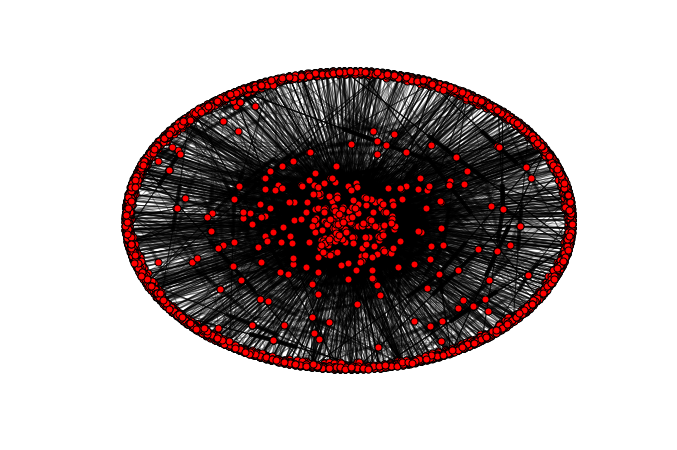
\includegraphics[width=1\textwidth]{img/findaslot_network_graph.png}
	\caption{Silk linkage rules for events in group 10's dataset.}
	\label{fig:link_event_g10}
\end{figure}

\subsection{LOD dataset}
- 25 Events with Location

\begin{lstlisting}[captionpos=b, caption=SPARQL query for getting Event with Location, label=lst:sparql, basicstyle=\ttfamily\small,frame=bt]

prefix event: <http://purl.org/NET/c4dm/event.owl#>

SELECT ?s ?p ?l
WHERE {
?s a event:Event .
{ 
bind(<http://vivoweb.org/ontology/core#hasGeographicLocation> as ?p) .
?s ?p ?lEn
}
UNION
{ 
bind(event:place as ?p) .
?s ?p ?lEn
}
?lEn rdfs:label ?l .
}

\end{lstlisting}

\section{Sub-graph extraction}
Event related graph

\subsection{Sub-graph analysis}
- new statistics

\section{Event finding}
- Query both datasets and report on instances gotten

\section{Conclusion}
Weight the differences between designing an ontology or cleaning existing ontologies.

\bibliographystyle{plain}
\bibliography{mybib}

\end{document}
